\section{Exponentials and $e$.}

As we implied before, $e^x$ is a horrendous notation which should be exiled from beginner-friendly explanations. Hence, we shall make a compromise to forget its existance until qualified to use it. We ask the reader to discard everything they know about exponentials up until secondary education.

Gathering what few understanding seems self-consistent, $a^q$ only makes sense when $a \in \mathbb{R}$ and $q \in \mathbb{Q}$ (one can question the nature of real numbers and what it means to multiply two together, but that lies far from the scope of this article). When $q \in \mathbb{N}$, exponentiation becomes the familiar \enquote{multiply $a$ times itself $q$ times}. However it is traditionally introduced that, because $a^b a^c = a^{b + c}$ and because $\sqrt[2]{a} \cdot \sqrt[2]{a} = a$, it is reasonable to say that $a^{\frac{1}{2}}\cdot a^{\frac{1}{2}} = a^{\frac{1}{2} + \frac{1}{2}} = a$, and hence that $a^{\frac{1}{2}} = \sqrt[2]{a}$. Extrapolating this and using similar properties, we generally say that $a^{\frac{b}{c}} = \sqrt[c]{a^b}$.

Note that at no point have we mentioned real numbers as exponents, and for good reason: they don’t make sense at all. How could one define $e^x$ to be a continuous function if only rational numbers are allowed?

\subsection{The area under $\frac{1}{t}$.}

Take the function $f(t) = \frac{1}{t}$ and let $A(x) = \int_1^x f(t) dt$ (Figure \ref{graph}). One can imagine this as a plane with axes $t$ and $y$ in which a function $f(t)$ is drawn. We establish a fixed point at $t = 1$ and draw a vertical line from the $t$ axis up until its intersection with $f(t)$. To its right, we have another vertical segment at $t = x$ which is also contained between the $t$ axis and the function’s graph. One can imagine $x$ and its line as moving freely through the $t$ axis, widening and shortening the \enquote{window} between the two vertical segments. With this notion in mind, the function $A(x)$ describes the value of the area of that window. Of course, this is just an integral.

\begin{figure}[H]
	\centering
	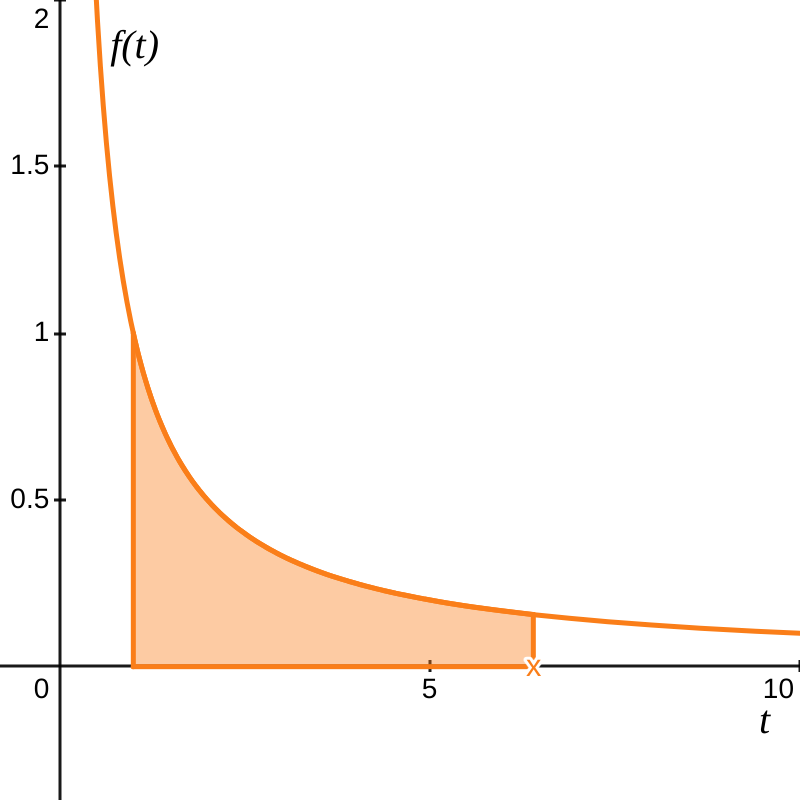
\includegraphics[width=\linewidth]{media/lnx.png}
	\caption{Graphical representation of the integral from $1$ to $x$ of the function $f(t) = \frac{1}{t}$. The variable $x$ can be thought of as a \enquote{slider} which changes how wide the integration window is. An interactive Desmos graph is available at \url{https://www.desmos.com/calculator/drhxhrnnr1}.}
	\label{graph}
\end{figure}

Note that what \enquote{varies} in $A(x)$ is $x$, in other words, that \enquote{slider} which changes how wide our window is. $t$ doesn't vary with $x$, it just defines the function. To clarify this, one might consider taking specific values of $x$. For example, $A(3) = \int_{1}^{3} f(t) dt$ means \enquote{the area encapsulated under the curve drawn by $\frac{1}{t}$ between $t = 1$ and $t = 3$}. This yields a real number with value $1.0986...$.

We \textbf{define} that area function to be the \textit{natural logarithm of $x$} (a name which might as well be meaningless for now), written as $\ln(x) := A(x) = \int_{1}^{x} \frac{1}{t} dt$. Because of the Fundamental Theorem of Calculus, $A'(x) = (\ln(x))' = \frac{1}{x}$ (it can also be proved using the Sandwich theorem). We also define $e$ to be the number that satisfies that $\ln(e) = 1$. 

\newpage

\subsection{Properties of the $\ln(x)$ function.}

Just by looking at the graph it is immediately obvious that for the $\ln(x)$ function to make sense, $x$ must be greater than $0$. We can analyse values between $0$ and $1$ by inverting the integration boundaries and the sign of the result. It's easy to see then that $\ln(x)$ is always an increasing function, and that for values between 0 and 1, its value will be negative. Furthermore, at $x = 1$, its area gets squished into nothingness, so $\ln(1) = 0$.

We can prove the following two properties:

\begin{itemize}
	\item $\ln(ax) = \ln(a) + \ln(x)$ for all $a, x \in \mathbb{R}^+$.
	\item $\ln(x^{\frac{p}{q}}) = \frac{p}{q} \ln(x)$ for all $\frac{p}{q} \in \mathbb{Q}$ and $x \in \mathbb{R}^+$.
\end{itemize}

\subsubsection{Proof of $\ln(ax) = \ln(a) + \ln(x)$.}

We start from taking the derivative of $\ln(ax)$:

$$(\ln(ax))' = \frac{1}{ax} \cdot a = \frac{1}{x} = (\ln(x))'$$

This implies that

$$(\ln(ax) - \ln(x))' = 0$$

meaning

$$\ln(ax) - \ln(x) = c \textrm{ (constant)}$$

To obtain the value of $c$, we can evaluate these functions at $x = 1$.

$$\ln(a) - \ln(1) = c \iff c = \ln(a)$$

That is to say

$$\ln(ax) = \ln(a) + \ln(x)$$

This method also works for proving that $\ln(\frac{x}{a}) = \ln(x) - \ln(a)$. Note that this works for \textit{every positive real number}. 

\subsubsection{Proof of $\ln(x^{\frac{p}{q}}) = \frac{p}{q} \ln(x)$}

Starting again from its derivative,

$$\ln(x^{\frac{p}{q}})' = \frac{1}{x^{\frac{p}{q}}} \frac{p}{q} x^{\frac{p}{q} - 1} = \frac{p}{q} \frac{1}{x} = \frac{p}{q} (\ln(x))'$$

Again, we substract the first and the last derivatives to get zero, meaning that $\ln(x^{\frac{p}{q}}) - \ln(x) = c$ with constant $c$. In this case, the constant turns out to be $c = 0$, leaving

$$\ln(x^{\frac{p}{q}}) = \frac{p}{q} \ln(x)$$

This is valid if $x > 0$ and if $\frac{p}{q} \in \mathbb{Q}$. Still, no real exponents to be found anywhere.

\subsection{The exponential function.}

By these properties, we can confidently say that:

$$\ln(e^2) = 2\ln(e) = 2$$
$$\ln(e^3) = 3\ln(e) = 3$$
$$\ln(e^4) = 4\ln(e) = 4$$
$$\ln(e^{q}) = q, \forall q \in \mathbb{Q}$$

Now we define the \textit{exponential function} to be the inverse of the natural logarithm function: $\exp(x) := \ln^{-1}(x)$. Think of the term \textit{exponential} as a name instead of an adjective. By this definition and by the previous results:

$$\exp(2) = \ln^{-1}(2) = e^2$$
$$\exp(3) = \ln^{-1}(3) = e^3$$
$$\exp(4) = \ln^{-1}(4) = e^4$$

It can be proved that the $\exp(x)$ function shares a lot of similarities with raising $e$ to a power in this regard. The usual properties of exponents transfer into this function.

$$\exp(a + b) = \exp(a\cdot b)$$
$$\exp(a \cdot b) = \exp(a)^b$$
$$\exp\left(\frac{1}{2}\right) = \sqrt{e}$$
$$\exp(-1) = e^{-1}$$

Because of this bizarre correlation, it is almost universal to write $\exp(x)$ as $e^x$. However, $\ln: (0, \infty) \to \mathbb{R}$, and hence $\exp: \mathbb{R} \to (0, \infty)$. In other words, we can evaluate $\exp(x)$ at irrational $x$ values. This isn't a problem for $\exp(x)$, but to say that $e^x$ can have an irrational power implies redefining what \enquote{power} even means.

In essence, we'll define every power with real exponent in terms of $\ln$ and $\exp$. Taking advantage of some notational abuse, we say that:

$$e^x := \exp(x)$$
$$a^x := \exp(x\cdot \ln(a)) = e^{x\cdot \ln(a)}$$

where $a\in \mathbb{R}^+$ and $x\in \mathbb{R}$. Note that $-a^x \in \mathbb{R}$, whereas $(-a)^x \in \mathbb{C}$. This is our first formal definition of $e$:

$$e := \exp(1) = \ln^{-1}(1) \iff \ln(e) = \int_{1}^{e} \frac{1}{t} dt = 1$$

\subsection{Other definitions of $e$.}

As with many things in math, what you define in one occasion turns up in other unexpected places. $e$ was originally discovered in the study of interest rates over different periods of time by Bernoulli.

$$\exp(x) = \lim_{n \to \infty} \left(1 + \frac{x}{n}\right)^n$$

$e$ is characteristic of those phenomena in nature where the rate of change of some variable depends on the value of that variable. Expressed through differential equations, $\exp(x)$ is the solution to:

\begin{equation}
	\begin{cases}
		f'(x) = f(x) \\
		f(0) = 1
	\end{cases}
\end{equation}

If we tried to examine $f$ through its Taylor expansion, we would get another definition for the exponential:

$$\exp(x) = \lim_{n \to \infty} \sum\limits_{k = 0}^{n} \frac{x^k}{k!}$$

\newpage
